%\bibliography{kilder.bib}









\subsection{Gravitation}

We will simulate the solar system with only the gravitational force affecting the planets.  Newton's gravitational law is stated in equation (\ref{eq:newton})\cite{uniphys}. It determines the gravitational force between two objects, where G is the gravitational constant ($6.67 \cdot 10^{-11} \rm{Nm^2/s^2}$), r is the distance between the planets, m is the mass of the object and M is the mass of the other object.

\begin{align}
	\vec{F_G}  =\frac{GmM}{\vec{|r|}^3}\vec{r}
	\label{eq:newton}
\end{align}

The gravitation force is an attractive force. It is worth noting that if the sun is at origo, the distance is simply the norm of the position vector of the planet. The mass of the sun has the special symbol $M_{\odot}$. 
\\
\\
For n objects the total gravitational force, $F_k$, for each object is: 


\begin{align}
	F_k = 
	\sum_{i = 1}^{N}
	\vec{F_i}  
	=
	\frac{Gm_km_i}
	{\vec{|r_k - r_i|}^3}
	(\vec{r_k} - \vec{r_i})
	(1 - \delta_{k,i})
	\label{eq:newton_all}
\end{align}

Where $\delta_{k,i}$ is the delta-function:

\begin{align*}
	\delta_{k,i} = \left\{\begin{matrix}
					1 & \text{if} \quad k =  i\\
					0 & \text{if} \quad k \neq i 
					\end{matrix}\right.
\end{align*}



We can use Newton's second law to determine the acceleration of the planet ($m_ka_k= F_{tot}$):

\begin{align}
	a_k
	=
	\sum_{i = 1}^{N}
	\frac{Gm_i}
	{|\vec{r_k} - \vec{r_i}|^3}
	(\vec{r_k} - \vec{r_i})
	(1 - \delta_{k,i})
	\label{eq:acceleration_all}
\end{align}














\subsection{Units}\label{sec:units}
As a famous person once said, "If you use seconds and meters you will not finish within the deadline".\footnote{Morten Hjorth-Jensen} Use of the units seconds and meters are impractical in this project. More suitable units are used. The mean distance between the earth and sun, 149 597 870 691 meter, is defined as one astronomical unit (au). For time, year is the unit.
These are the units that will be used in this project. 
\\
\\
We can now express the gravitational constant with these units. To do this we use the formula for the acceleration of a circular orbit, $\frac{v^2}{r}$. Combine this with the equation (\ref{eq:newton}) and Newton's second law, we get: 

\begin{align*}
	\frac{v^2}{r} =
	\frac{GM_{\odot}}{\vec{|r|}^3}\vec{r} 
	\implies 
	G
	=
	\frac{v^2 r}{M_{\odot}} = \frac{\rm{au} (2\pi \cdot \rm{au/year})^2}{M_{\odot}}
	=
	\frac{4\pi^2}
	{M_{\odot}} \rm{au^3/year^2}
\end{align*}

\pagebreak

Applying this to equation (\ref{eq:acceleration_all}), we get: 

\begin{align}
	a_k
	=
	\sum_{i = 1}^{N}
	4 \pi \frac{m_i}{M_{\odot}}
	\frac{(\vec{r_k} - \vec{r_i})}
	{|\vec{r_k} - \vec{r_i}|^3}
	(1 - \delta_{k,i}) \rm{au^3/year^2}
	\label{eq:acceleration_all_au}
\end{align}

Note that if you pick $M_\odot = 4 \pi$, then you get G = 1 and a planet's mass become $m_i = 4\pi \frac{m_{i_{kg}}} {M_{\odot_{kg}}}$.







\subsubsection{Escape velocity}\label{sec:escape-velocity}

Later in the project we are asked to find the escape velocity by trial and error. This question is basicly, when does the earth have enough kinetic energy to escape the gravitational potential from the sun. The potential is equal to $\int_0^\infty F_G dr$. For a given planet with only the sun in the solar system the integral is from r to $\infty$. This is shown in equation (\ref{eq:escape-velocity}).  


\begin{align}
E_k =\int_r^\infty \frac{GmM}{\vec{|r|}^2} d\vec{r}
\label{eq:escape-velocity}
\end{align}

Let's solve it: 

\begin{align*}
	&E_k =\int_r^\infty -\frac{GmM_\odot}{\vec{|r|}^2} d\vec{r}
	\\
	&\frac{1}{2}mv^2 = GmM_\odot \int_r^\infty -\frac{1}{\vec{|r|}^2} d\vec{r}
	\\
	&\intertext{G = 1, see section \ref{sec:units} for explanation.}
	\\
	&\frac{1}{2}v^2 = M_\odot \int_r^\infty -\frac{1}{\vec{|r|}^2} d\vec{r}
	\\
	&\frac{1}{2}v^2 = M_\odot \left[ \frac{1}{\vec{|r|}} \right]_r^\infty
	\\
	&v^2 = 2M_\odot \frac{1}{\vec{|r|}}
	\\
	&\intertext{r = 1, see section \ref{sec:units} for explanation.}
	\\
	&v = \sqrt{8\pi^2}
	\\
	&v \approx 8.8857 \rm{au/year}
\end{align*}










\subsection{The perihelion precession of mercury}\label{sec:perihelion}

The distance between a satellite in orbit and the center of this orbit (focal point) will fluctuate. The point at which the satellite is closest to its orbital center is called the perihelion, while the one furthest away is called the aphelion. For a simple, Newtonian, two body system the elliptical orbit does not move or change and so the perihelion (or aphelion) doesn't either. However, when more satellites are introduced they affect each other in such a way as to change the location of the perihelion over time. This is called a perihelion precession. In our experiment we consider only the two body system of sun/Mercury and use a modified gravitational law that takes relativistic effects into account. This way we know that any precession we get is caused solely by relativistic effects. Furthermore, a precession of $\theta = 43''$ would account precicesly for the deviation between the classical prediction and observed values and ultimately strengthen Einsteins theory of general relativity.\\

In our case the new and improved gravitational law can be stated through the following formula

$$F_G = \frac{GM_{Sun}M_{Mercury}}{r^2}\qty[1 + \frac{3l^2}{r^2c^2}]$$

Here we recognize the traditional components of the classical gravitational law while also noting the addition of a new term that contains a constant, $c$ (the speed of light), and a variable, $l$ the magnitude of Mercury's orbital angular momentum per unit mass

$$
l = \abs{\vec{r}\times \vec{v}}
$$

It is trivial to show the following relation between angle and coordinates using simple trigonometry
$$\tan \theta = \frac{y_p}{x_p}$$

\begin{figure}[H]
	\centering
	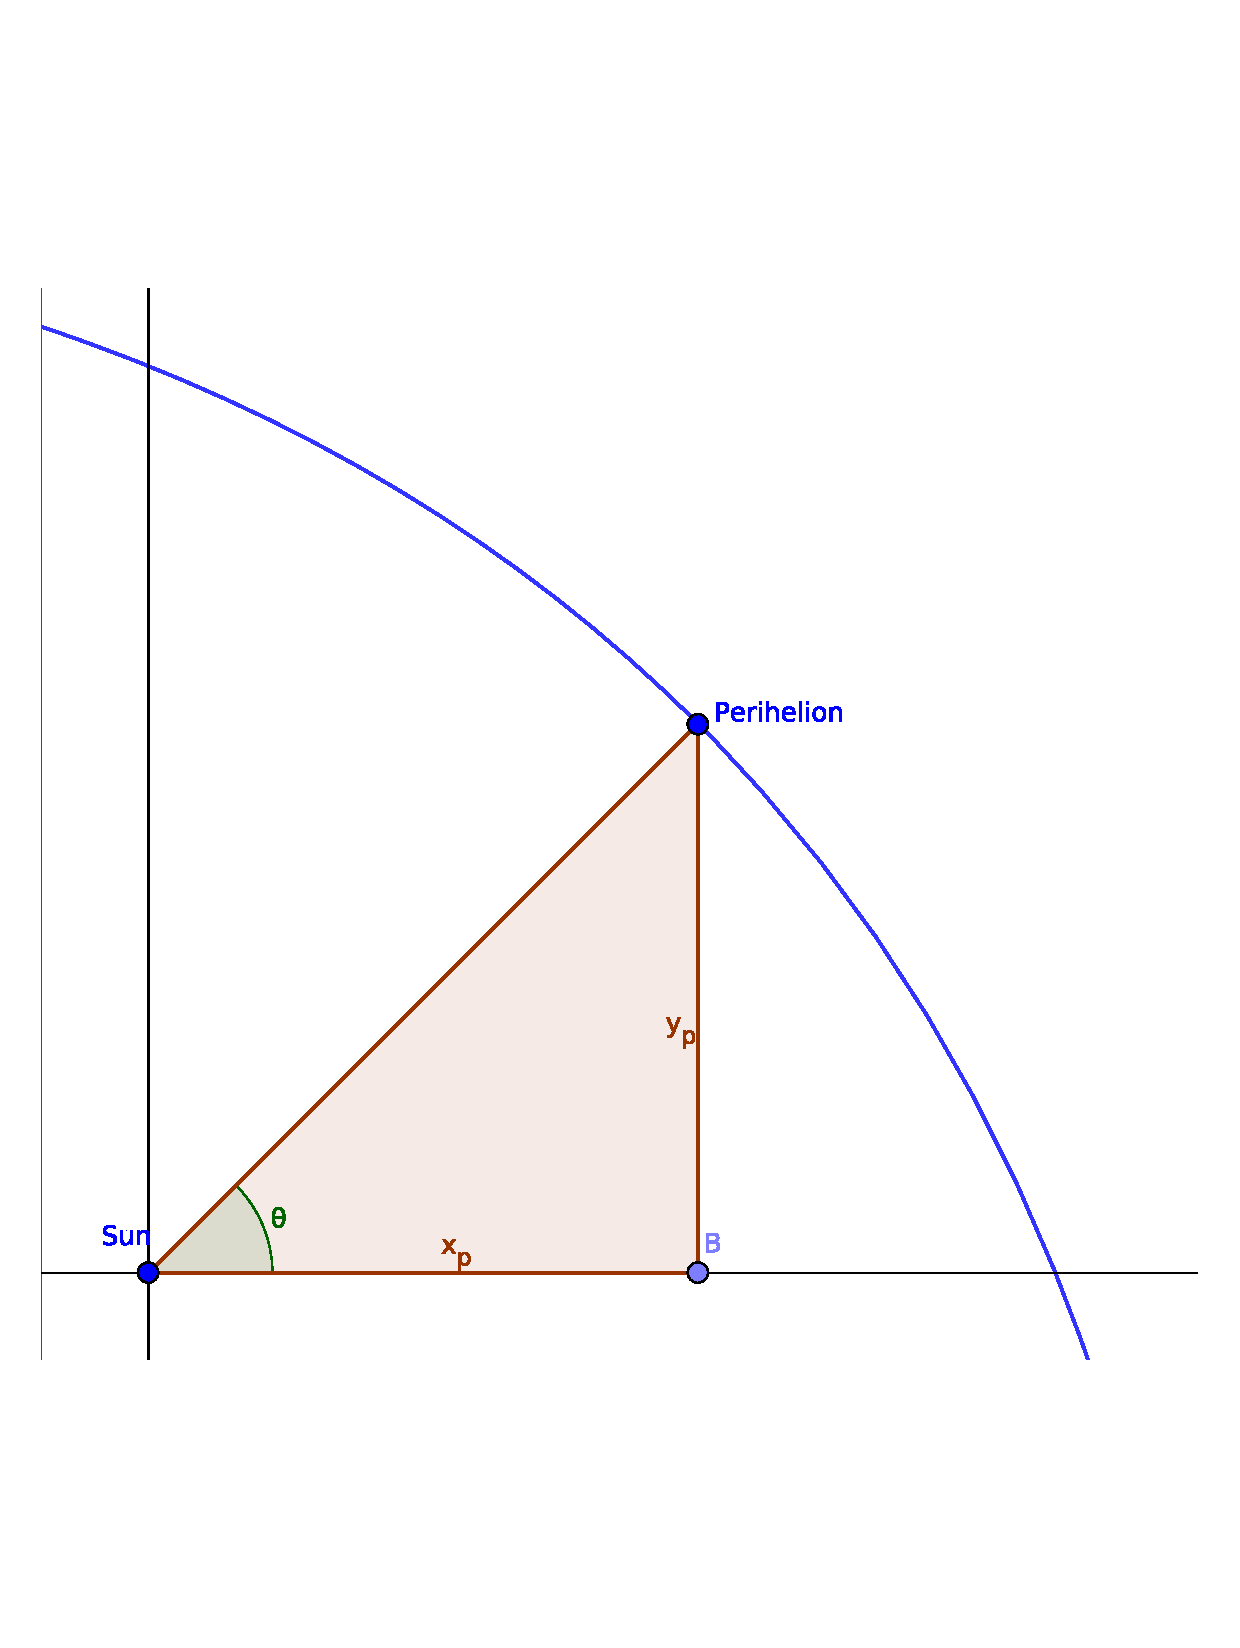
\includegraphics[width = 0.4\linewidth]{theory/bilder/figure.pdf}
	\caption{The figure shows the angle ($\theta$) and coordinates $(x_p,y_p)$ for the perihelion of Mercury. And with the formula $\tan \theta = \frac{opposite}{adjacent}$}
\end{figure}






\subsection{Numerical methods}

Equation (\ref{eq:acceleration_all_au}),initial conditions and the standard relations between position, velocity, acceleration determine the orbit of the planets. These equations are for x,y and z direction, written out you get a coupled set of differential equations. This set is near impossible to solve analytically. It might be impossible. We will use numerical methods to solve this set. More specifically we will use the Forward Euler method and the Velocity-Verlet method. A given $t_i$ is equal to $t_0 + ih$, where $h = (t_{0} + t_{n})/n $.













\subsubsection{Forward Euler}

Both methods use a Taylor polynomial approximation to solve the set of differential equation. The Forward Euler uses the first order Taylor polynomial. With $r'(t) = v(t)$ and $v'(t) = a(t)$ the Forward Euler method results in: 
 
\begin{align}
	&\vec{r_i}(t+h) \approx \vec{r_i}(t) + h \vec{v_i}(t)
	\\
	&\vec{v_i}(t+h) \approx \vec{v_i}(t) + h \vec{a_i}(t)
\end{align}

Discretized version. i is the object number and j is the time step:

\begin{align*}
	&\vec{r_{i,j+1}} \approx \vec{r_{i,j}} + h \vec{v}_{i,j}
	\\
	&\vec{v_{i,j+1}} \approx \vec{v_{i,j}} + h \vec{a}_{i,j}
\end{align*}

The error for a first order taylor polynomial goes as $\mathcal{O}(h^3)$ \cite{compphys}. This is the error for each step. The error is accumulated for each step and will therefore be proportional to h. 













\subsubsection{Velocity-Verlet}

You guessed it, this is the second order Taylor polynomial. As I said the Velocity-Verlet method is based on a Taylor polynomial approximation. And this is the second order. 

\begin{align}
	&\vec{r_i}(t+h) \approx \vec{r_i}(t) + h \vec{v_i}(t) + \frac{1}{2} h^2 a(t)
	\\
	&\vec{v_i}(t+h) \approx \vec{v_i}(t) + h \vec{a}(t) + \frac{1}{2} h^2 \vec{a}'(t)
	\label{eq:verlet}
\end{align}

Since we have no formula for the derivative of a, we use the approximation: 

\begin{align*}
	\vec{a}'(t) \approx \frac{\vec{a}(t+h) - \vec{a}(t)}{h}
\end{align*}

We simply update the position first. We keep the old acceleration and calculate the acceleration at the new position.  Using this and equation (\ref{eq:verlet}) we get: 

\begin{align*}
	&\vec{v_i}(t+h) \approx \vec{v_i}(t) + h \vec{a}(t) + \frac{1}{2} h(\vec{a}(t+h) - \vec{a}(t))
	\\
	&\vec{v_i}(t+h) \approx \vec{v_i}(t) + \frac{1}{2} h(\vec{a}(t+h) + \vec{a}(t))
\end{align*}

Discretized version. i is the object number and j is the time step:
\begin{align*}
	\\
	&\vec{r}_{i,j+1} \approx \vec{r}_{i,j} + h \vec{v}_{i,j} + \frac{1}{2} h^2 a_{i,j}
	\\
	&\vec{v}_{i,j+1} \approx \vec{v}_{i,j} +\frac{1}{2} h(\vec{a}_{i,j+1} + \vec{a}_{i,j})
\end{align*}


The error for a first order taylor polynomial goes as $\mathcal{O}(h^2)$ \cite{compphys}. This is the error for each step. The error is accumulated for each step and will thereby be proportional to $h^2$. This is one order of magnitude better, then the Forward Euler method. 
















